\section{Methodology}\label{sec:method}
\subsection{Visibility and initial fragments}
Before correlation, the receiver checks that the evidence ledger is contiguous, has one availability entry per alert, agrees with alert-level availability, and contains no private fields. At cutoff $T=100$, it keeps only arrived alerts and claims whose two endpoints are eligible. The initial pass groups same-source and process-tree fragments, then considers available lineage references. Host, account, and size guards apply to the components at that stage. The later claim verifier does not go back and certify every pair made within a source. This matters when interpreting the zero false-pair result: it was observed in the holdout, not guaranteed by the verifier's logic.

\subsection{Original independent attestation}
For each proposed relationship, the baseline inspects a bundle of claims. To join two fragments it needs one original process claim, one original authentication claim, and one original network claim, all from different upstream roots and all available by $T$. Endpoint and event identities, host, account, process parent, session, and flow fields must agree. The event-time check is $t_b\geq t_a-3$ and $|t_b-t_a|\leq25$ minutes. A copy of an original observation does not supply a missing family. Finally, the two current components must overlap on host and account and contain at most 100 alerts after union.

The root and visibility checks are necessary conditions:
\begin{equation}\label{eq:gate}
\left|\{\rho(c):c\in B_r,\;c\text{ original}\}\right|=3,\qquad
\max_{c\in B_r}t_{\mathrm{available}}(c)\leq T.
\end{equation}
The two conditions in (\ref{eq:gate}) are only part of the decision. Identity, context, event time, and component guards must also pass. On failure the verifier records a reason and makes no union. It checks each token against original alert fields; a newly enlarged group cannot serve as a new witness for the next token. Group membership is nevertheless transitive after independently checked unions, so one final group may contain several fragments.

\subsection{Constrained endpoint fallback}
The candidate revisits just one failure reason: \texttt{missing\_family}. If the process claim is absent, it may use original endpoint observations alongside one original authentication and one original network-flow claim. The two claims must have different roots and be available by minute 100. The endpoints must be original, have different source and observation IDs, and share an endpoint-origin root distinct from both claim roots. Host, account, event timing, process parent, session, and flow must agree between endpoints and claims. The existing component guards still apply. Thus the endpoint context fills the missing process-family role; it cannot excuse a contradiction, a late claim, or another failure. Figure~\ref{fig:verify} shows the branches.
\begin{figure*}[t]\centering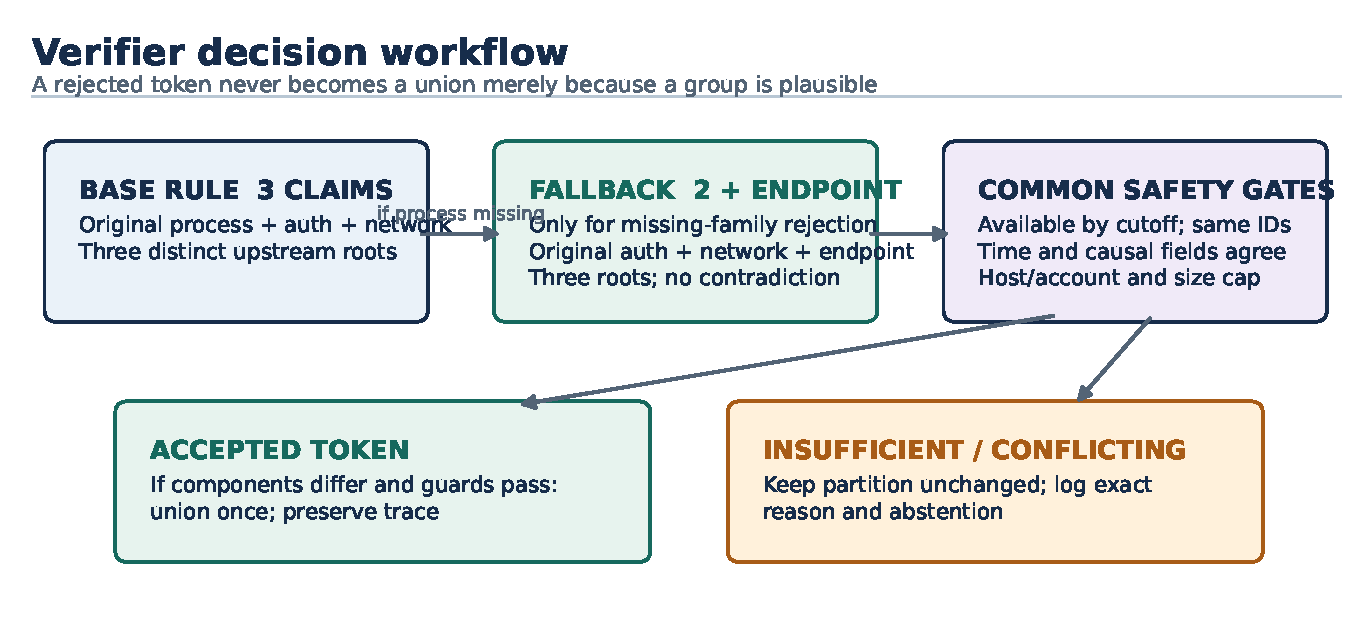
\includegraphics[width=.88\textwidth]{figures/verification_methodology.pdf}\caption{Frozen verifier workflow. The baseline requires original process, authentication and network claims from three distinct roots. Only \texttt{missing\_family} can trigger the fallback: original authentication and network claims plus a distinct original endpoint root. Identity, event-time, availability, causal fields, component context and size gates still apply. Failure leaves the partition intact. Evaluator truth is unavailable to prediction.}\label{fig:verify}\end{figure*}

\subsection{Decision semantics and component state}
Claim validity and permission to merge are separate checks. A valid token may point to alerts already in one component; then there is nothing to join. It may also pass its claim checks but fail because the proposed combined group would exceed 100 alerts or the components have no host/account overlap. Existing groups stay intact in either case. Bundles are processed in sorted order, with union--find tracking the additional verified joins. The three-root requirement counts the original observations for a token, not alerts accumulated in its component.

Table~\ref{tab:decisions} gives logical decision cases, not extra measured experiments. An authentication claim copied into a second derived record still has one upstream root; a future-dated claim cannot be used at the decision cutoff even if its underlying event happened earlier. A contradiction is not repaired by the endpoint rule. Conversely, an absent process claim can be substituted only after the exact authentication/network and endpoint conditions above succeed. These distinctions explain why missing evidence may cause abstention while conflicting evidence blocks an otherwise plausible relationship.
\begin{table*}[t]\centering\footnotesize\caption{Verifier decision cases implied by the frozen code. Examples illustrate rule behavior and are not counts from the holdout.}\label{tab:decisions}\begin{tabularx}{\textwidth}{@{}p{0.25\textwidth}Yp{0.24\textwidth}@{}}\toprule Case & Gate implicated & Effect on grouping\\\midrule Derived copy offered as another witness & Original-claim and distinct-root checks & No added union\\ Two original claim families, process absent & Exact authentication/network and endpoint fallback checks & Union only if every fallback and component guard passes\\ Claim arrives after cutoff & Evidence availability check & Claim unavailable for this decision\\ Event or causal identifier disagrees & Endpoint and claim consistency checks & No added union\\ Verified token exceeds component cap & Current component size check & No added union\\\bottomrule\end{tabularx}\end{table*}

\subsection{Grouping and scoring}
Both arms rank by source depth: $1.2$ times maximum severity, $0.7$ times maximum asset criticality, $0.55$ times distinct event types among source representatives, and $0.7$ times the number of distinct sources capped at 10. The code first constructs a dictionary keyed by source ID and retains one representative alert per source. The frozen baseline adds one point per accepted token whose left endpoint is in the group. The candidate uses the same bonus coefficient of one and includes fallback unions. Groups are sorted by descending score and then first alert identifier. A group never becomes recoverable merely because its rank changes; Figure~\ref{fig:groups} separates grouping from top-20 retrieval.
For group $G$, let $D(G)$ denote the code's one-alert-per-source representatives, $s(a)$ and $c(a)$ the alert severity and criticality, $E(D)$ the distinct event types in those representatives, and $U(G)$ the accepted tokens whose left endpoint belongs to $G$. The implemented score in both primary arms is
\begin{equation}\label{eq:score}
F(G)=1.2\max_{a\in D(G)}s(a)+0.7\max_{a\in D(G)}c(a)
+0.55|E(D(G))|+0.7\min\{|D(G)|,10\}+|U(G)|.
\end{equation}
The fallback can change both $G$ and $U(G)$, so a changed rank is not isolated evidence of a superior ranking function. The fixed ranking expression is a deterministic heuristic, not a learned probability of incident severity.
\begin{figure}[ht]\centering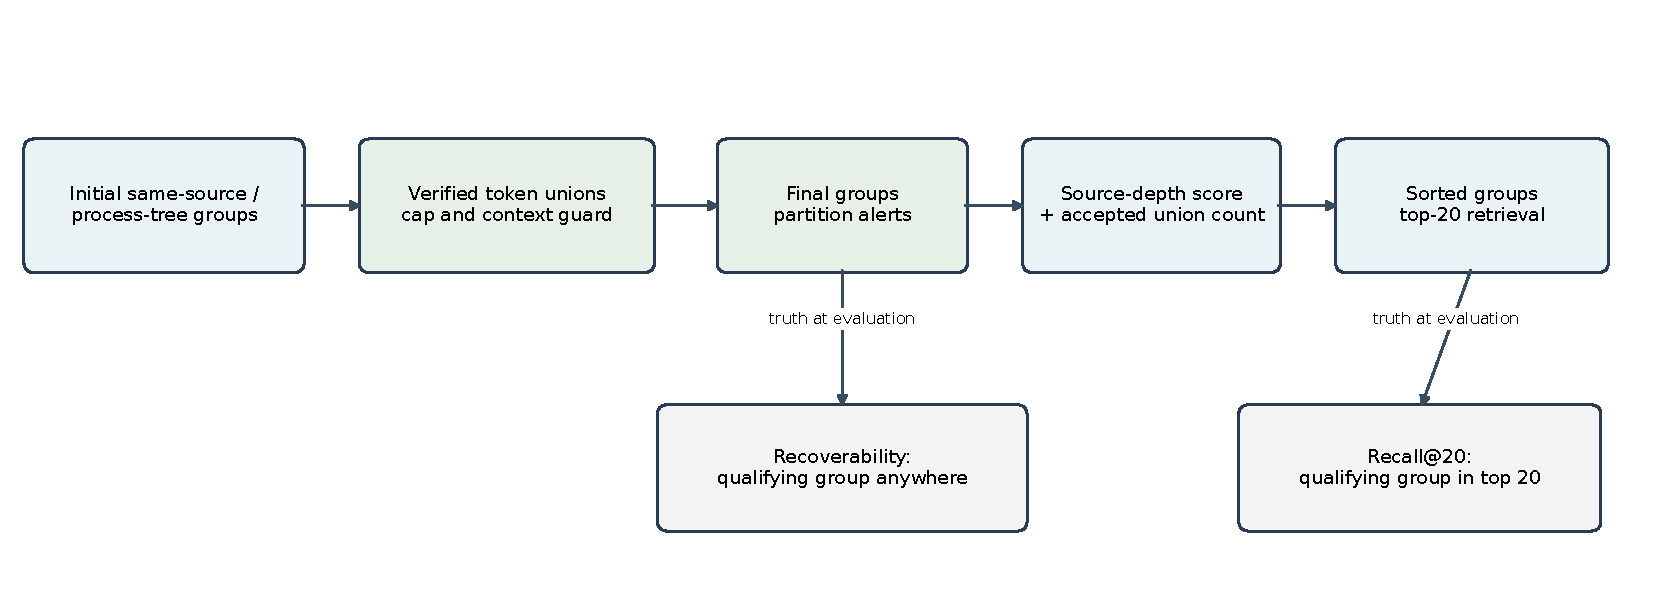
\includegraphics[width=\linewidth]{figures/reconstruction_prioritization.pdf}\caption{Initial fragments and accepted evidence-token unions form the final partition. Scoring orders these fixed groups. The evaluator separately checks whether an expert incident has a sufficiently complete and pure group anywhere (recoverability) and whether one appears within the first 20 (Recall@20); ranking cannot create a missing group.}\label{fig:groups}\end{figure}
